\documentclass[11pt]{article}
\usepackage[utf8]{inputenc}
\usepackage{hyperref, amsmath, amssymb, amsthm, graphicx, fancyvrb, enumitem, titlesec, setspace, float, fancyvrb, minted}
\usepackage[dvipsnames]{xcolor}
\usepackage[top=1in, bottom=1in, left=1.25in, right=1.25in]{geometry}

\titleformat{\section}{\normalfont\bfseries}{}{0em}{}
\titlespacing*{\section}{0pt}{1.5ex plus .2ex minus .2ex}{0.8ex plus .1ex}

\begin{document}
\noindent Andre Winkel \hfill \today \\
\rule{\textwidth}{0.4pt}

\begin{center} \large {\textbf{Lab 2}} \\[0em] {EE141, Digital Signal Processing, Fall 2025} \end{center}

\section{Problem 1: Reviewing and verifying properties of the DTFT}
In this problem, we consider the discrete time Fourier transform given by
\begin{equation} \notag
    X(e^{j\omega}) = \sum_{n=-\infty}^{\infty}x[n]e^{-j\omega n}.
\end{equation}
We also consider that if $x[n]$ is a causal sequence, this sum reduces to
\begin{equation}
    X(e^{j\omega}) = \sum_{n=0}^{\infty}x[n]e^{-j\omega n},
\end{equation}
and we can further truncate the above sum to
\begin{equation}
    X(e^{j\omega}) \approx \tilde X(e^{j\omega}) \triangleq \sum_{n=0}^{\infty}x[n]e^{-j\omega n}
\end{equation}
if $x[n]$ decays to zero as $n \to \infty$.
For this problem, we let $x[n]=0.8^nu[n]$ and $y[n]=0.7^n\cos(\frac{\pi n}{6})u[n]$.

\begin{enumerate}[label=\textbf{\alph*)}, leftmargin=2.6em]
    \item Solving analytically for $x[n]$, we observe
    \begin{equation} \notag
        X(e^{j\omega}) = \sum_{n=0}^{\infty}0.8^n e^{-j\omega n}
    \end{equation}
    as $x[n]$ is a causal signal, shown in (1). We can further simplify to 
    \begin{equation} \notag
        X(e^{j\omega}) = \sum_{n=0}^{\infty}(0.8e^{-j\omega})^n,
    \end{equation}
    where we observe this as a converging sum, as $a=0.8<\infty$.
    Continuing with our idea of infinite geometric series, we can simplify this even further to
    \begin{equation} \notag
        X(e^{j\omega}) = \frac{1}{1-0.8e^{-j\omega}}.
    \end{equation}
    We can then use this in MATLAB to solve for $X(e^{j\omega})$ in an analytical manner, using our
    \texttt{w = linspace(-pi, pi, K)} where $K = 500$.

    \item Picking a large enough $N$ s.t. $0.9^N\approx 0$ (used $N=50$), we use MATLAB to numerically compute 
    $X(e^{j\omega_k})$ using (2).

    \item Plotting the analytical and numerical solutions, we observe the following:
    \begin{figure} [H]
        \centering
        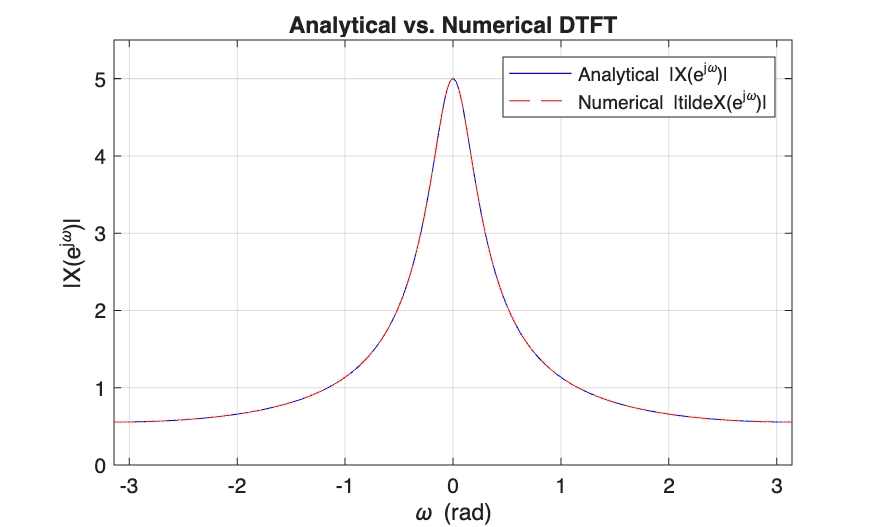
\includegraphics[width=0.6\linewidth]{partc.png}
    \end{figure}

    \item Doing the same for $y[n]$, we observe the following plot:
    \begin{figure} [H]
        \centering
        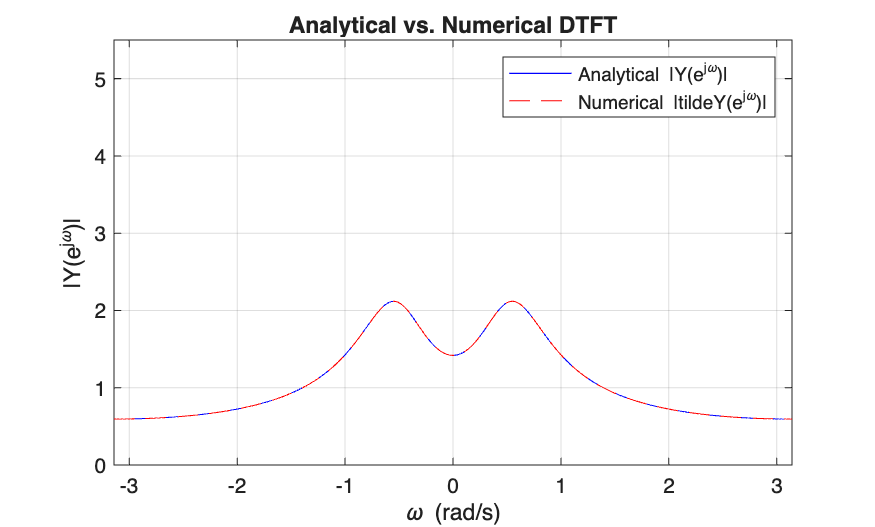
\includegraphics[width=0.6\linewidth]{partd.png}
    \end{figure}

    \item We now let $z[n] = 2x[n] + 3y[n]$. Analytically computing $Z(e^{j\omega_k})$ and numerically computing
    $\tilde Z(e^{j\omega_k})$ using the same $\omega_k$ as in the previous parts, we observe the following
    magnitude and sum plots:
    \begin{figure} [H]
        \centering
        \includegraphics[width=0.4\linewidth]{parte1.png}
        \includegraphics[width=0.4\linewidth]{parte2.png}
    \end{figure}


\end{enumerate}

\end{document}